\documentclass[a4paper]{article}

\usepackage{INTERSPEECH2020}


\usepackage{array}
\newcolumntype{P}[1]{>{\centering\arraybackslash}p{#1}}
\newcolumntype{M}[1]{>{\centering\arraybackslash}m{#1}}


\usepackage{subcaption}
\usepackage[hidelinks]{hyperref}
\usepackage[style=ieee]{biblatex}
\addbibresource{mybib.bib}

\title{Spoken Keyword Spotting}
\name{Vineeth S}
\address{
  Indian Institute of Science, Bengaluru
}

\begin{document}
\maketitle

\begin{abstract}

Spoken Keyword Spotting is the task of identifying predefined words (called as keywords) from speech. Keyword spotting forms the foundation of the current trends of virtual assistants such as Google Home and Amazon Alexa. Due to its always-on nature, KWS systems have stringent constraints of power and memory budget. We explore using a hybrid system consisting of a Convolutional Neural Network and a Support Vector Machine for KWS task. The code is available at  \url{https://github.com/vineeths96/Spoken-Keyword-Spotting}.

\end{abstract}
\noindent\textbf{Index Terms}: keyword spotting, convolutional neural networks, support vector machine


\section{Introduction}

Rapid developments and research in the areas of voice-based interaction with machines has tremendously influenced the heavy adaptation of these technologies into everyday life. With the development of devices such as Google Home, Amazon Alexa and Smartphones, speech is increasingly becoming a more natural way to interact with devices. However, always-on speech recognition is generally not preferred due to its energy inefficiency and network congestion that arises due to continuous audio stream from millions of devices to the cloud. Processing such a large amount of audio stream will require more time and adds to the latency and can have privacy issues.

Keyword Spotting (KWS) provides an efficient solution to all the above issues. Modern day voice-based devices first detect predefined keyword(s) --- such as "OK Google", "Alexa" --- from the speech locally on the device. On successfully detecting such words, a full scale speech recognition is triggered on the cloud (or on the device). Since the KWS system is always-on, it is highly preferred to have low memory footprint and computation complexity, but with high accuracy and low latency. We explore using a hybrid system that can fit into the above setting, guaranteeing the desired results.


\section{Related work}

Traditional approaches for KWS are based on Hidden Markov Models with sequence search algorithms. With the advances in deep learning and increase in the amount of available data, state-of-the-art KWS has been replaced by deep learning based approaches due to their superior performance\cite{6854370}. Several attempts have been made using Deep Neural Networks (DNNs) and Convolutional Neural Networks (CNNs) to perform KWS task adhering to constraint budgets on memory and power\cite{Tabibian}. CNNs turn to be a befitting candidate for KWS task, because they capture translational invariance with far fewer parameters than DNNs by averaging the outputs of hidden units in different local time and frequency regions\cite{Sainath2015}. CNNs are also capable of embedding speech by transforming them from input representations to meaningful representations\cite{8639036}. 

We use the Google Speech Commands dataset which contains $65,000$ WAVE audio files of thirty words recorded by people with different demographics\cite{gsc}. Each recording is about one-second long and contains a single word recorded at $16$KHz sampling rate. The dataset is categorized into $6798$ validation recordings, $9916$ test recordings and rest as training recordings.


\section{KWS System}

Out of the words available in the Google Speech Commands dataset, we choose the word \textit{Marvin} to be our keyword. With minimal modifications and retraining, any available word(s) in the dataset can be configured to be a keyword(s). There are $1758$ positive recordings (of Marvin) and $62,982$ negative recordings (of other words) in dataset. Clearly, the dataset is highly imbalanced and direct training with this data might not produce desired results. The possibility of overfitting the positive data samples in such a case cannot be overlooked.

To provide a suitable solution with this setting, we look at a hybrid system --- consisting of a Convolutional Neural Network (CNN) and a Support Vector Machine (SVM). We train the CNN model to be a feature extractor that embeds the input into a suitable representation that properly captures the relevant information. We then train an One Class SVM (OCSVM), popularly used for outlier detection, with these embeddings as input. OCSVM is an unsupervised outlier detector particularly used in scenarios where there are huge imbalances in the dataset.

We shall look at the implementation and training of KWS system. The KWS system is implemented in Python using \textit{Tensorflow} framework and \textit{scikit-learn} library. Fig \ref{fig:feature_embedder} shows the implemented KWS system. The input to the system is the log Mel Filterbank energies of the speech signal calculated with a window of length $25ms$ and stepsize $10ms$. We use \textit{Tensoflow Dataset} API for efficient handling of inputs --- generating input features on-the-fly --- since loading the entire dataset into memory would require high resources.

\begin{figure}[h]
	\centering
	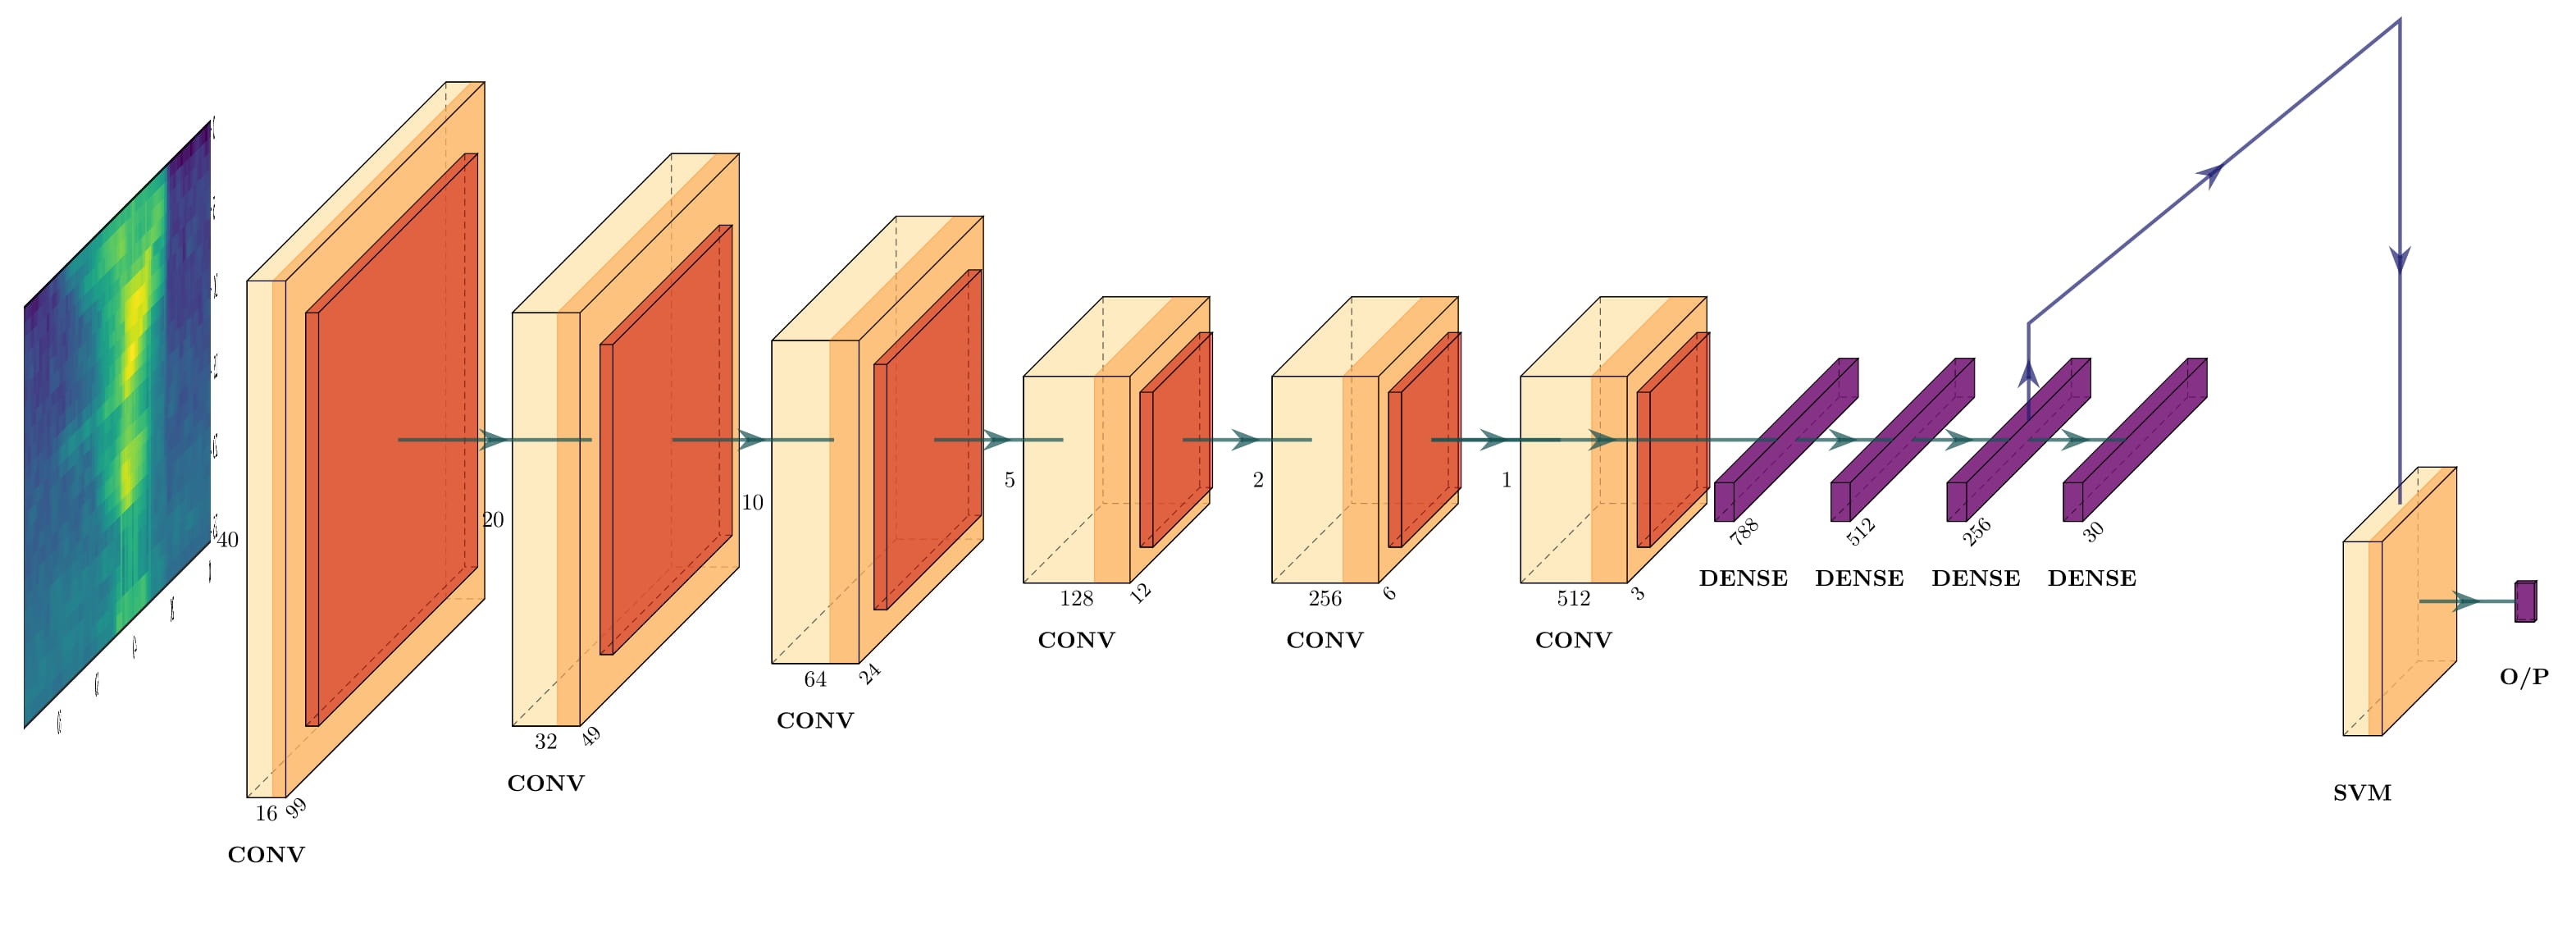
\includegraphics[width=1\linewidth]{../results/kws3.jpg}
	\caption{KWS architecture}
	\label{fig:feature_embedder}
\end{figure}

First, we train a thirty-word classifier based on CNN architecture above using the training files in the dataset. The model achieved an training accuracy of $96.59\%$ and validation accuracy of $95.56\%$. The deep network can be interpreted as a ``black box" that transforms the input representations into meaningful representations, with which the final layer perform a classification. Since we have good performance in classification, we can safely assume that the model learns the proper representations for the input. We consider the output of the $256$ dimensional penultimate dense layer (marked with arrow on Fig \ref{fig:feature_embedder}) as an \textit{embedding} of the input feature. 

We train the OCSVM with these embedding as input. We do not use the entire training set for this purpose. We use the validation set for this purpose. Since OCSVM is an outlier detector, it needs only the positive samples to learn the maximum margin detector. The performance of OCSVM is highly dependent on its hyperparameters values. To obtain the best-performing OCSVM, we tune the hyperparameters using \textit{scikit-optimize} library. Fig \ref{fig:hyper_tune} shows the F1 score variation over iteration count with different tuning methods. We choose the best performing \textit{gp\_minimize()} function for tuning. This tuning method approximates the cost function values
(here, - F1 Score) as a Gaussian process and minimizes it using Bayesian optimization. This method is far less expensive compared to other methods and performs empirically well.

\begin{figure}[htb]
	\centering
	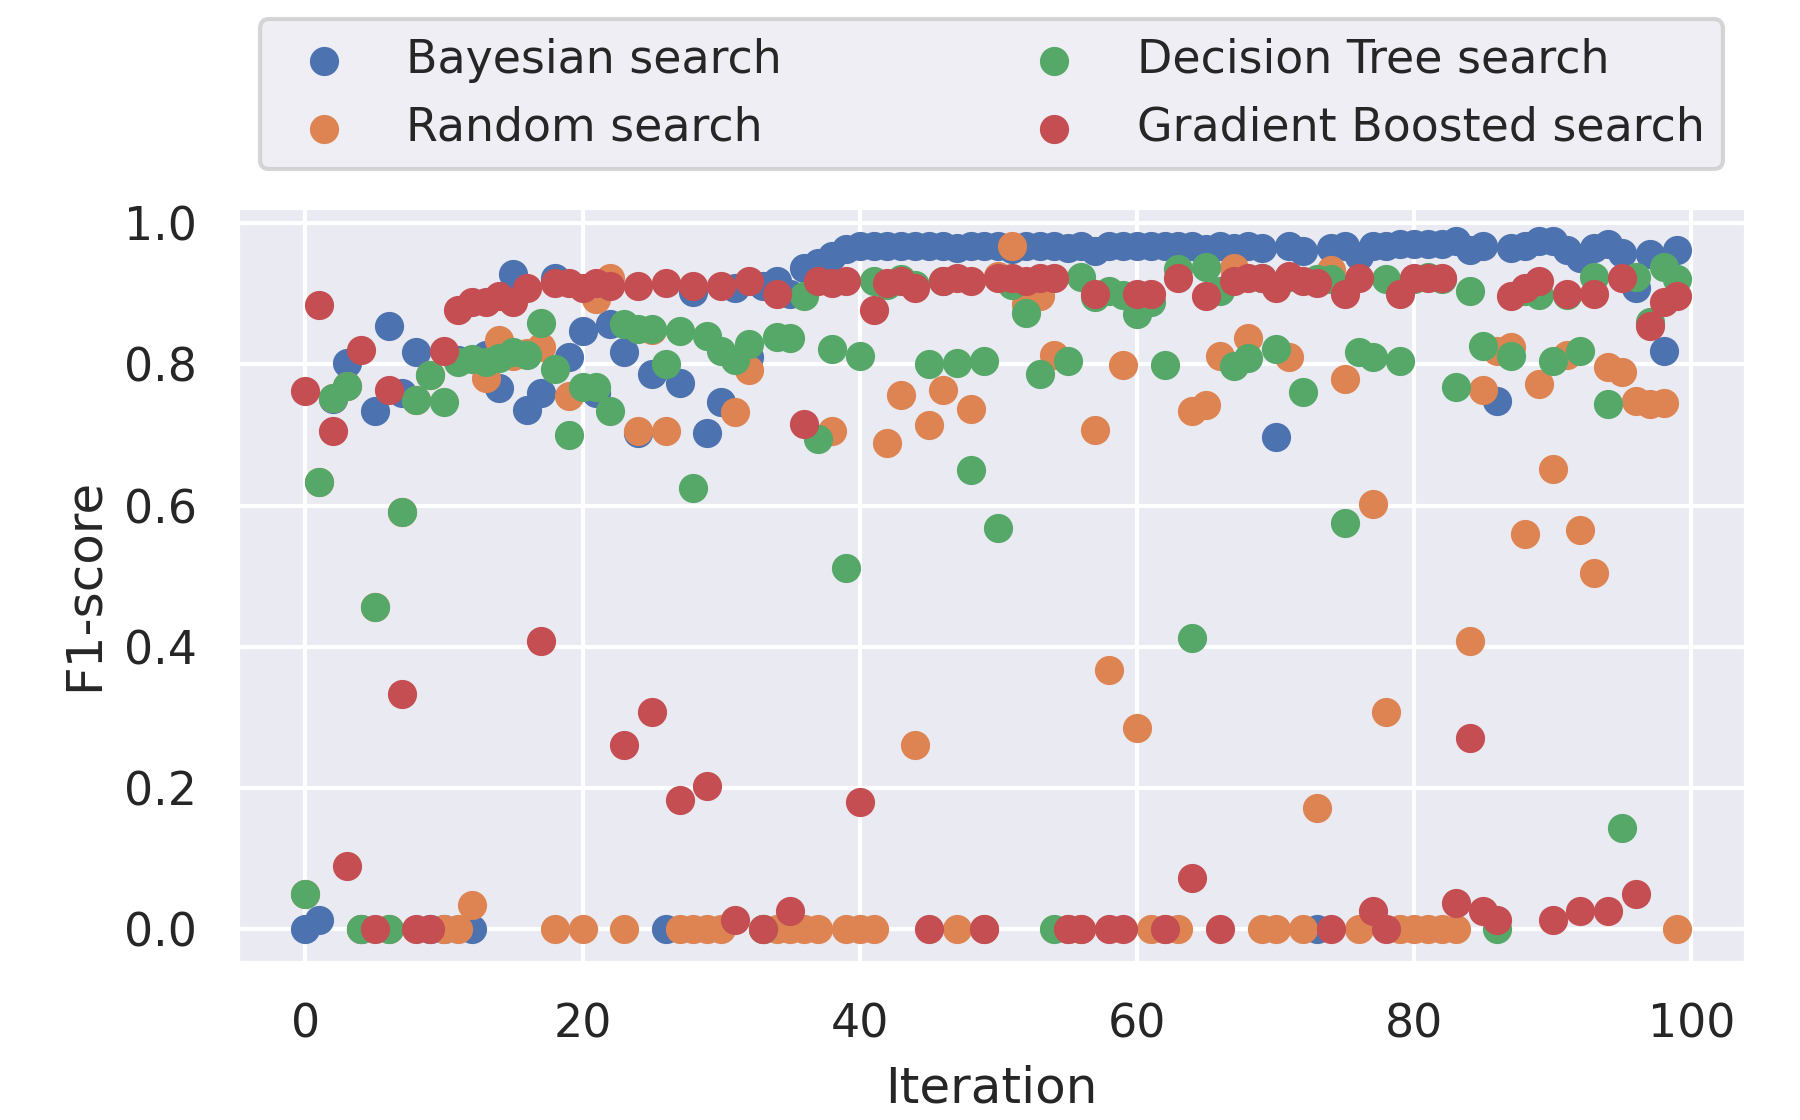
\includegraphics[width=1\linewidth]{../results/marvin_tuning.png}
	\caption{Hyperparameter tuning}
	\label{fig:hyper_tune}
\end{figure}

We train the OCSVM with positive samples from validation set with the hyperparameters set with the optimal values. We then evaluate our model on the test set, whose results are summarized below in Fig \ref{fig:results}. We can observe that we have a high value of detection and low value of false alarm which are typically desired of a KWS system.

\begin{figure}[htb]
	\centering
	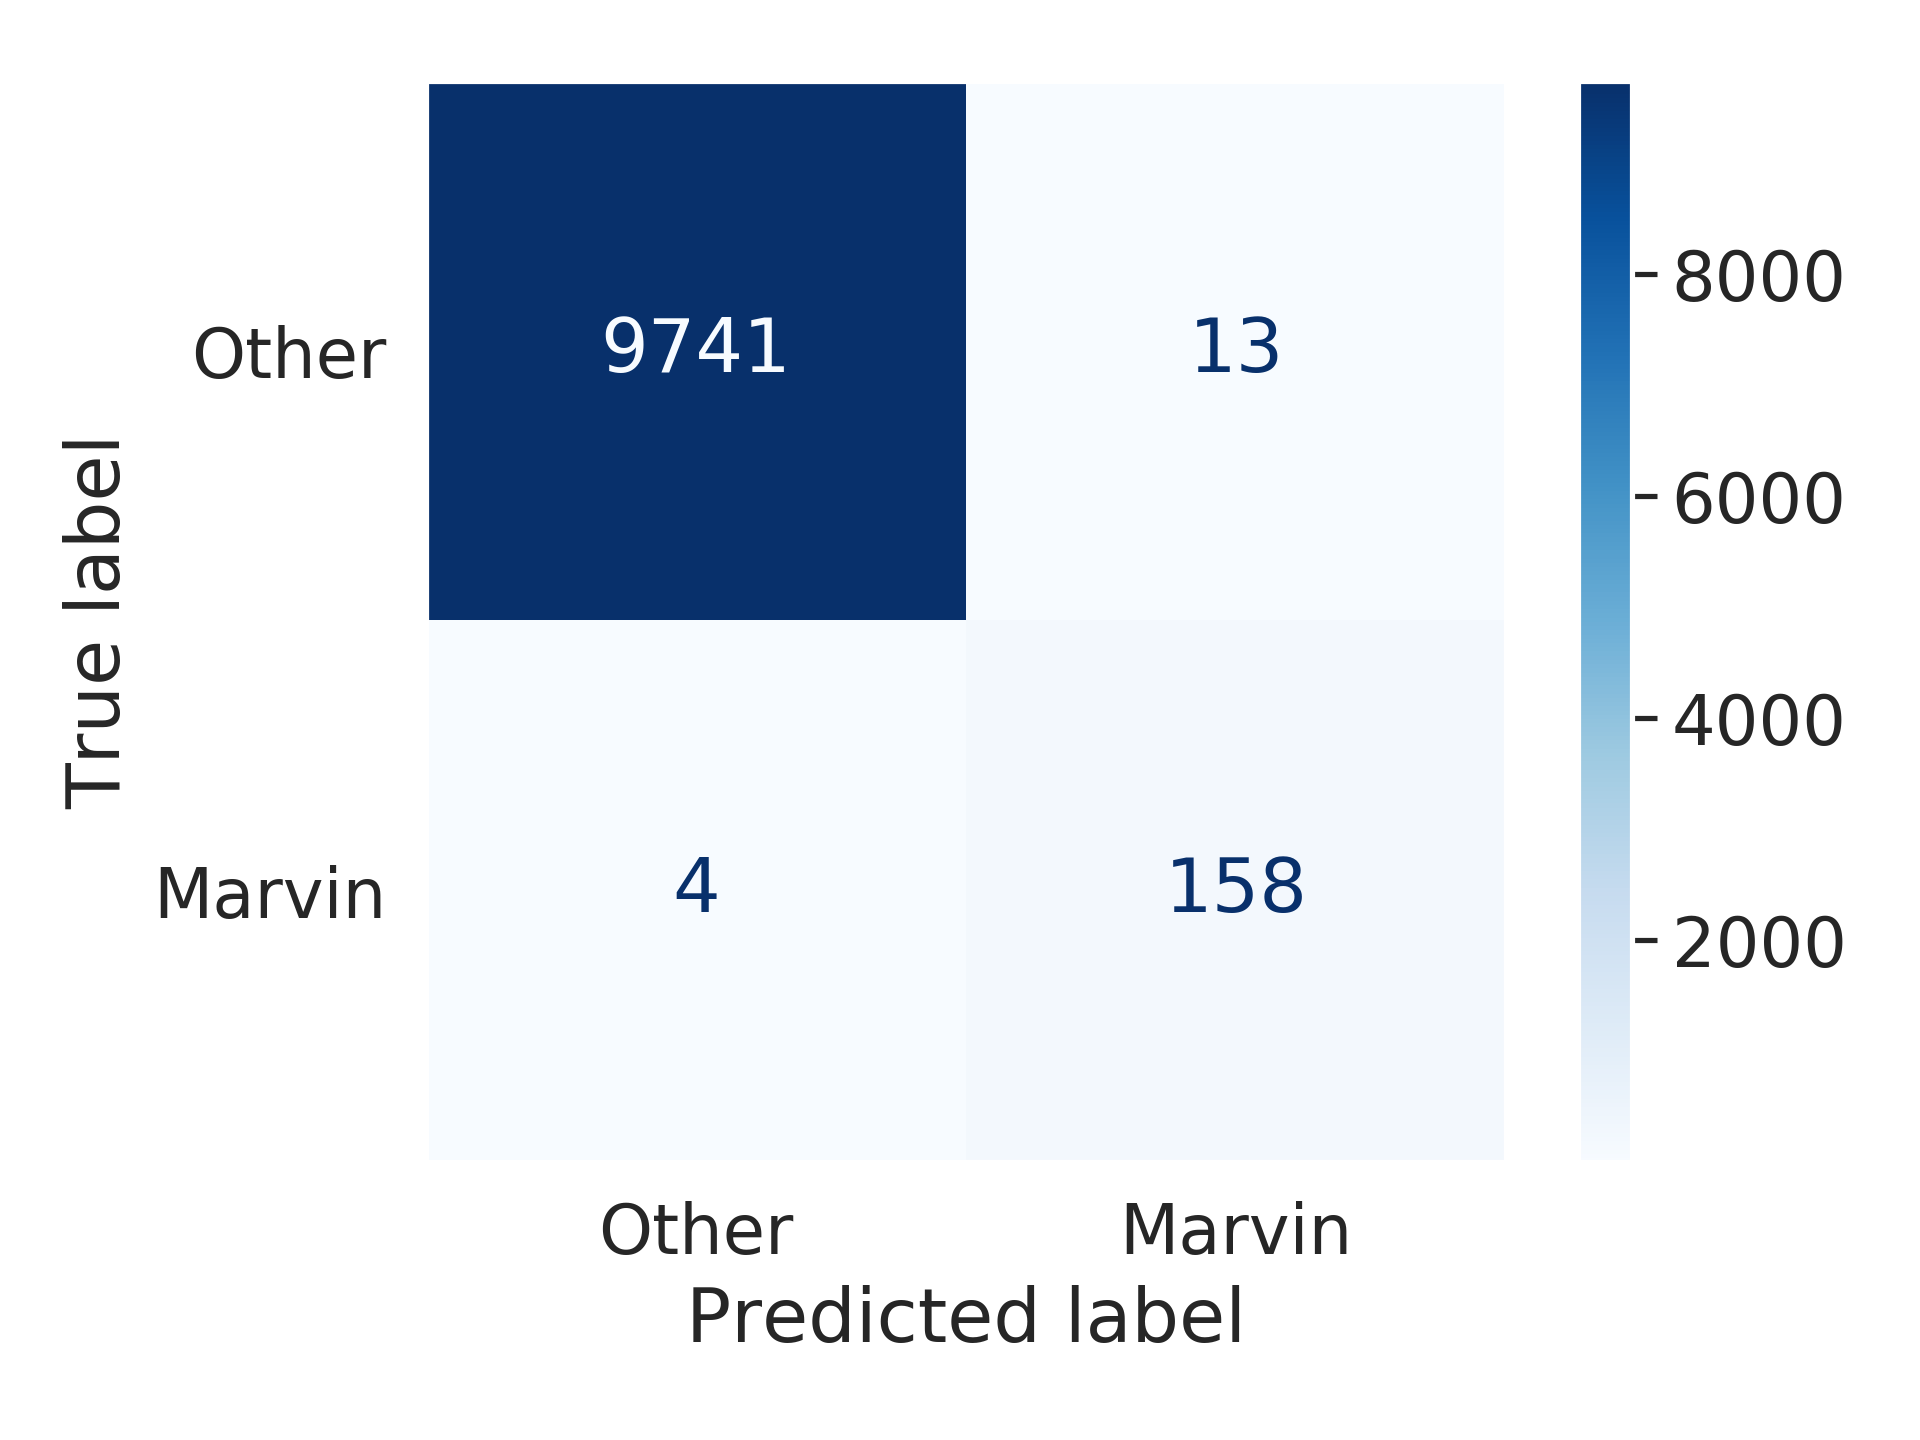
\includegraphics[width=0.8\linewidth]{../results/marvin_cm_without_noise.png}
	\caption{Test set: Confusion Matrix}
	\label{fig:results}
\end{figure}

Fig \ref{fig:ROC} shows the Receiver Operating Characteristics (ROC) and Fig \ref{fig:PR} shows the Precision Recall graph of the classifier. We can observe that the area under the curve for both curves are 1, which is desirable, but the use of these graphs for a imbalanced set is debatable. Table \ref{tab:KWS} shows the various performance metrics for the hybrid KWS system developed. The definitions in \cite{Tabibian, Section 2.2} have been used for the calculation of these metrics (where applicable).

As mentioned earlier, any available word(s) in the dataset can be configured as a keyword(s) by retraining just the SVM. Though we have used a limited vocabulary set of thirty words, this CNN-OCSVM model performs without any noticeable pitfalls in continuous speech comprising of out-of-vocabulary (OOV) words. This can be tested by executing the \textit{stream\_audio} script in the associated code repository. Moreover, this performance can be enhanced using large vocabulary datasets such as Mozilla Common Voice. Research also shows that there are methods by which even OOV word(s) could be configured as keyword(s), when the dataset is large enough.

\begin{figure}
	\begin{subfigure}[b]{0.49\columnwidth}
		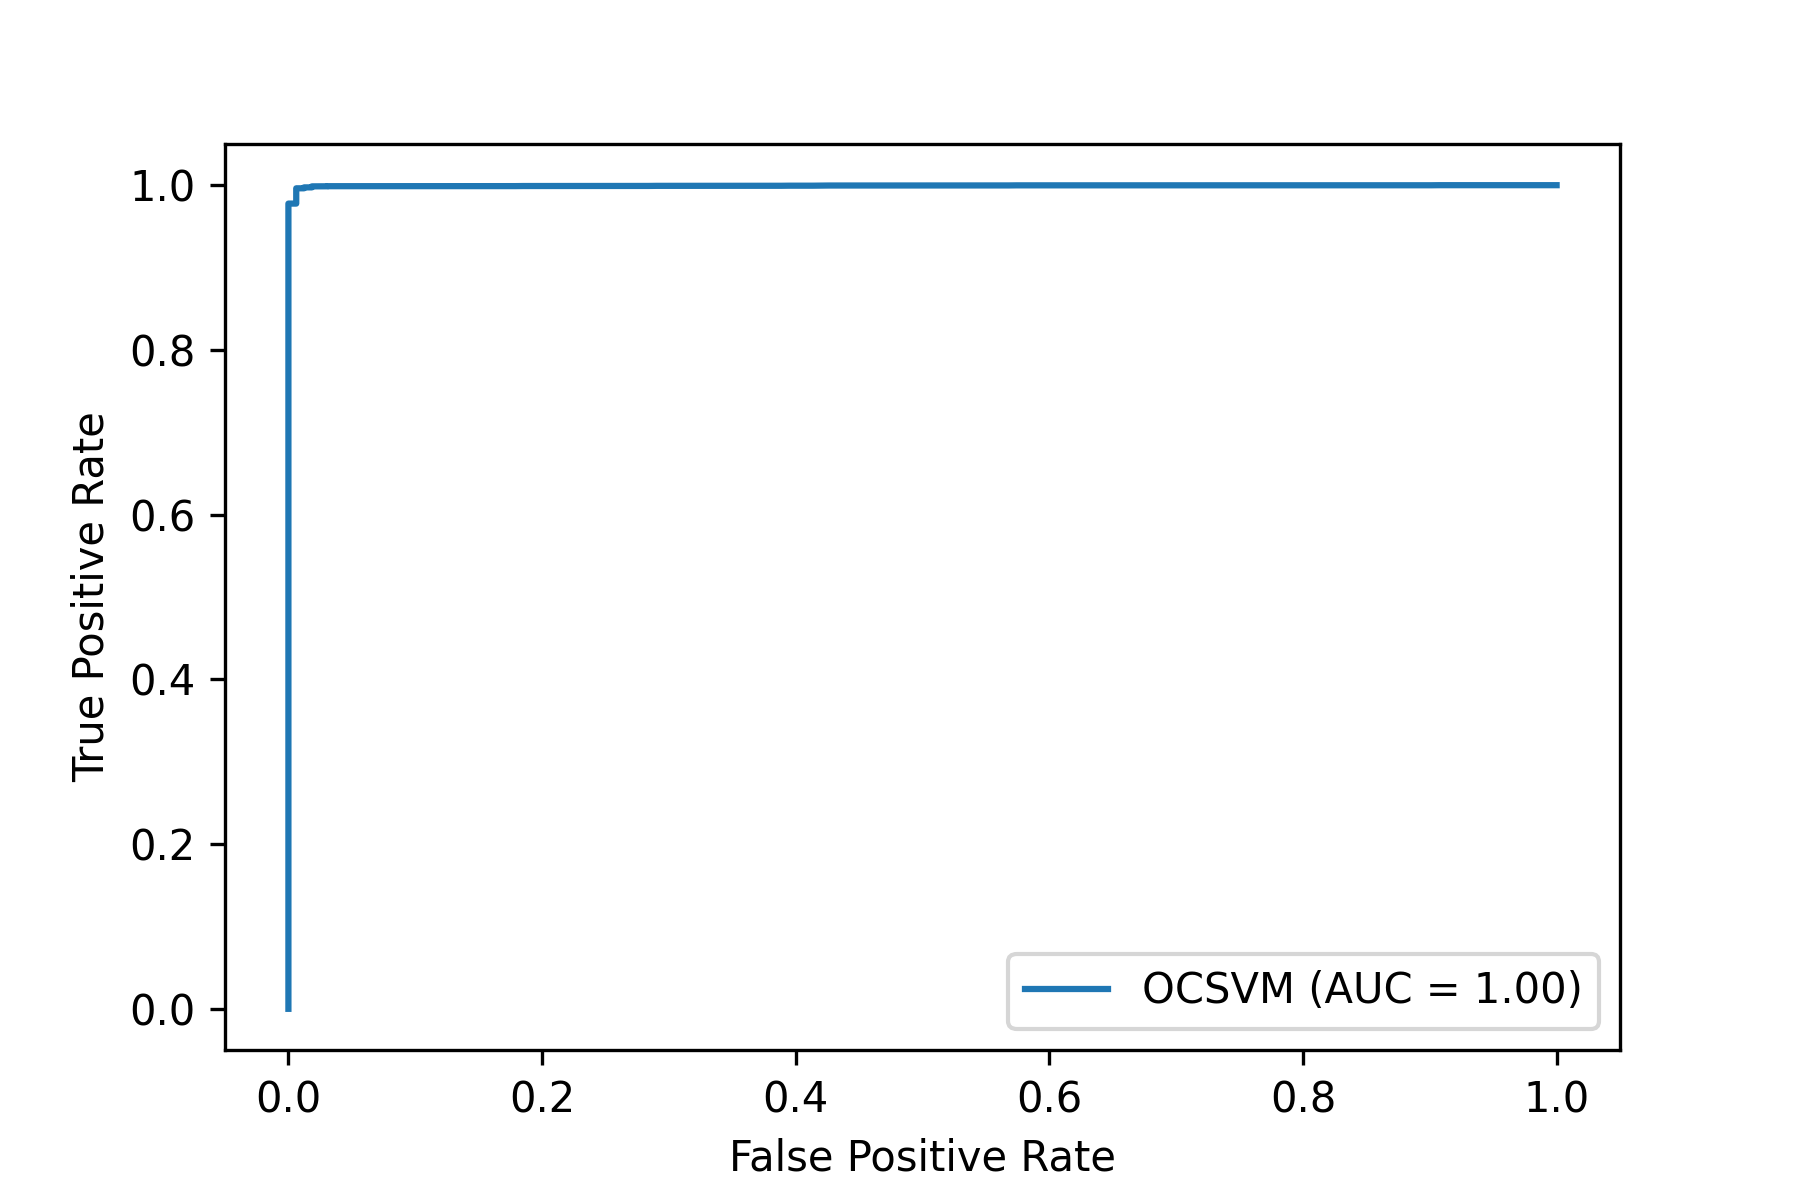
\includegraphics[width=\linewidth]{../results/ROC.png}
		\caption{ROC Curve}
		\label{fig:ROC}
	\end{subfigure}
	\hfill %%
	\begin{subfigure}[b]{0.49\columnwidth}
		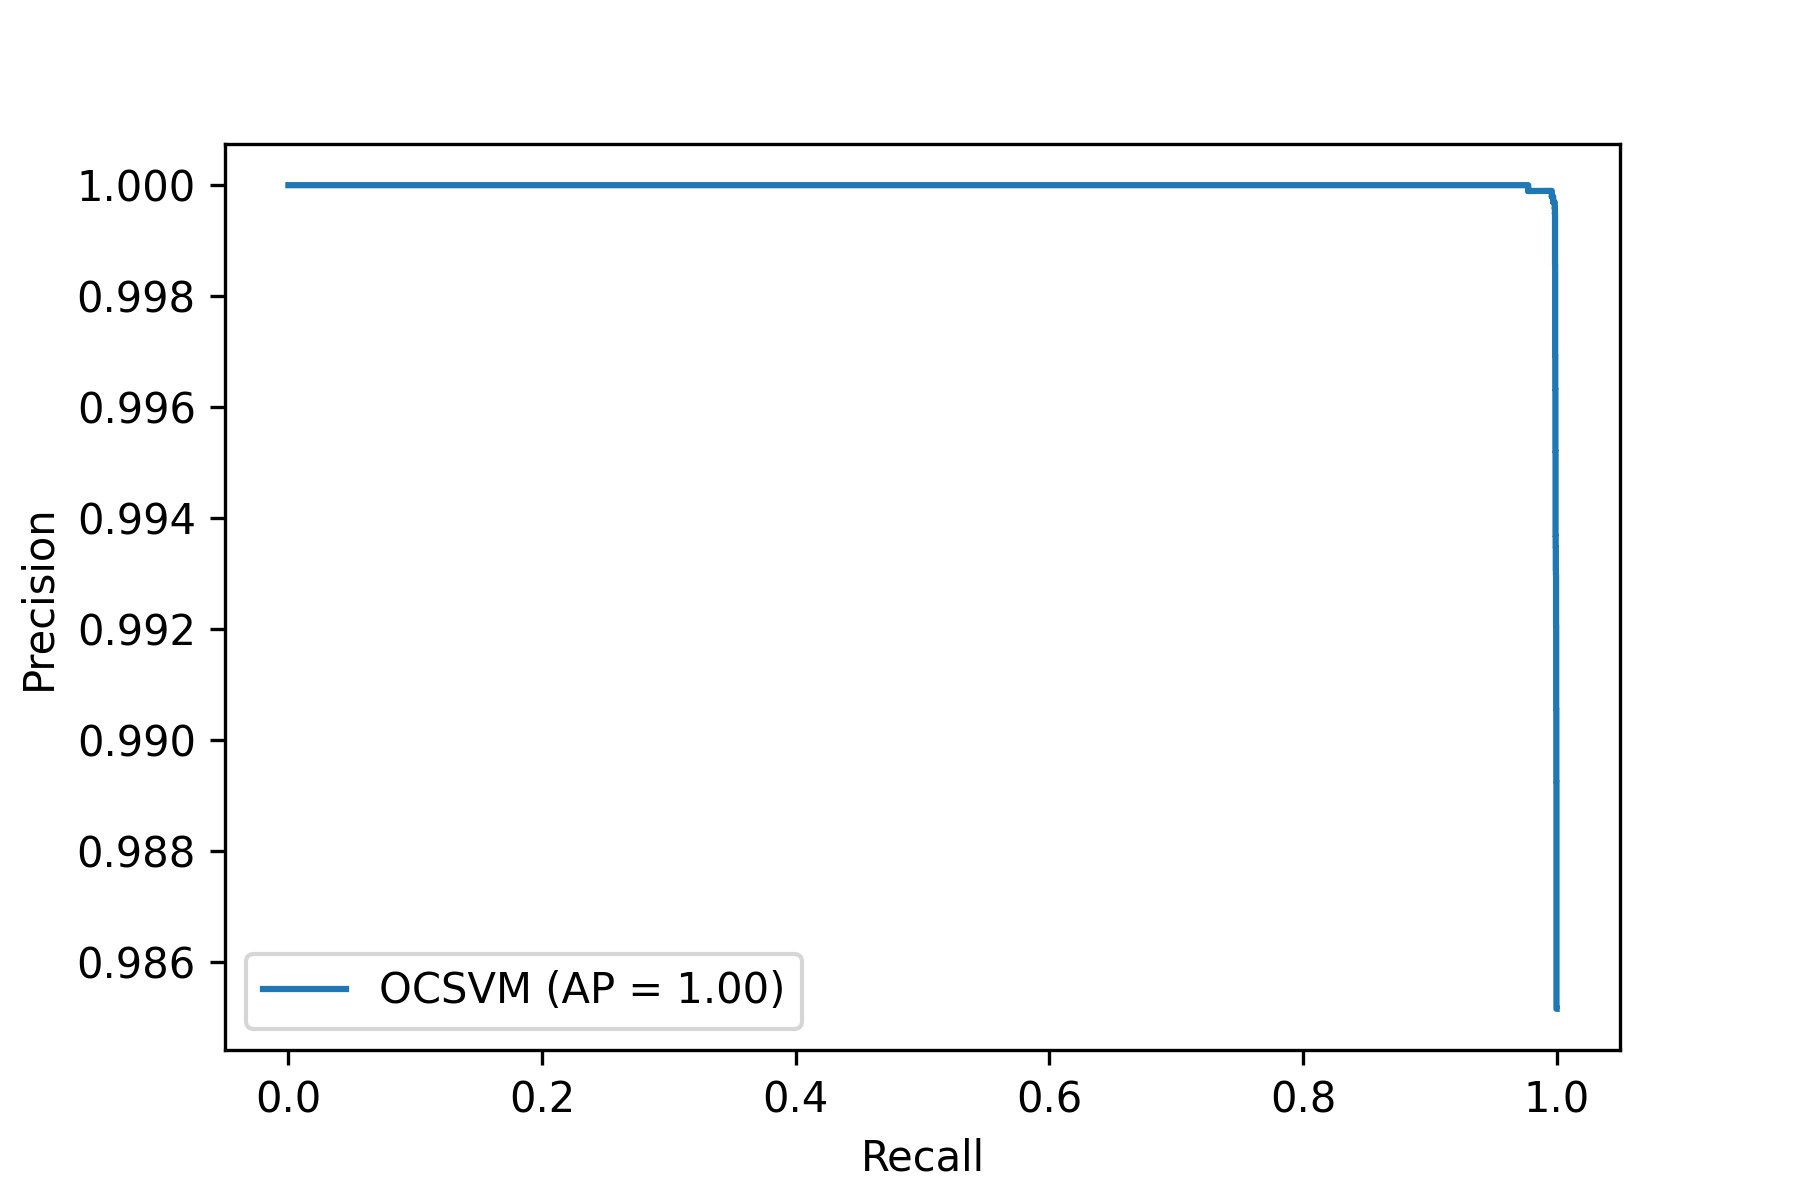
\includegraphics[width=\linewidth]{../results/PR.png}
		\caption{Precision Recall Curve}
		\label{fig:PR}
	\end{subfigure}
\end{figure}

 
\begin{table}[h]
  \caption{KWS System Performance Metrics}
  \label{tab:KWS}
  \centering
  \begin{tabular}{|M{4.5cm}|M{2.5cm}|}
    %\toprule
    \hline
    Model size 		 					& $11.4$MB            \\ \hline
    Model size (Quantized) 				& $978$KB             \\ \hline
	Real Time Factor (RTF)			 	& $1.7$ms             \\ \hline
	Accuracy 		 					& $0.9995$            \\ \hline
	Precision			 				& $0.9942$            \\ \hline
	Recall (True Detection Rate) 		& $0.9770$            \\ \hline
	F1 Score			 				& $0.9855$            \\ \hline
	Matthews Correlation Coefficient 	& $0.9853$            \\ \hline
	False Alarm Rate (FAR)			 	& $0.0001$            \\ \hline
	False Alarm per Hour (FA/Hr)		& $0.0003$            \\ \hline
	True Rejection Rates (TRR)		 	& $0.9998$            \\ \hline
	False Rejection Rates (FRR)			& $0.0229$            \\ \hline
	True Rejection Rates (TRR)		 	& $0.9998$            \\ \hline

    \hline
    %\bottomrule
  \end{tabular}
\end{table}


\section{Conclusions}

A small footprint reconfigurable CNN-OCSVM based KWS system is proposed in this work. The raw performance numbers shows that this model outperforms many of the models in the literature. However, a direct comparison is not meaningful because of the differences in the datasets and the actual keywords. To prove this claim a lot of further work is necessary, such as performance analysis under noise and far-field conditions.

\section{References}
\printbibliography[heading=none]

\end{document}
